\documentclass[12pt, a4paper, oneside]{ctexart}
\usepackage{amsmath, amsthm, amssymb, bm, color, graphicx, geometry, hyperref, mathrsfs,extarrows, braket, booktabs, array}
\setmainfont{Times New Roman}  % 设置英文字体
\setsansfont{Calibri}
\setmonofont{Consolas}

\linespread{1.4}

%\geometry{left=2.54cm,right=2.54cm,top=3.18cm,bottom=3.18cm}
\geometry{left=1.84cm,right=1.84cm,top=2.18cm,bottom=2.18cm}
\newenvironment{problem}{\par\noindent\textbf{题目. }}{\bigskip\par}
\newenvironment{solution}{\par\noindent\textbf{解答. }}{\bigskip\par}
\newenvironment{note}{\par\noindent\textbf{注记. }}{\bigskip\par}

% 一些宏定义
\def\bd{\boldsymbol}
\def\disp{\displaystyle}
\def\sign{\text{sign}}
\def\wtd{\widetilde}
\def\bR{\mathbb{R}}
\def\wdh{\widehat}
\def\L{\mathcal{L}}
\def\add{\vspace{0.5ex}}  % 增加行间距
\def\del{\vspace{-3.5ex}}  % 减少行间距

% 基本信息
\newcommand{\RQ}{\today} % 日期
\newcommand{\km}{数值分析} % 科目
\newcommand{\bj}{强基数学002} % 班级
\newcommand{\xm}{吴天阳} % 姓名
\newcommand{\xh}{2204210460} % 学号
\newcommand{\XH}{59} % 序号

\begin{document}

%\pagestyle{empty}
\pagestyle{plain}
\vspace*{-15ex}
\centerline{\begin{tabular}{*6{c}}
    \parbox[t]{0.25\linewidth}{\begin{center}\textbf{日期}\\ \large \textcolor{blue}{\RQ}\end{center}} 
    & \parbox[t]{0.15\linewidth}{\begin{center}\textbf{科目}\\ \large \textcolor{blue}{\km}\end{center}}
    & \parbox[t]{0.2\linewidth}{\begin{center}\textbf{班级}\\ \large \textcolor{blue}{\bj}\end{center}}
    & \parbox[t]{0.1\linewidth}{\begin{center}\textbf{姓名}\\ \large \textcolor{blue}{\xm}\end{center}}
    & \parbox[t]{0.15\linewidth}{\begin{center}\textbf{学号}\\ \large \textcolor{blue}{\xh}\end{center}}
    & \parbox[t]{0.1\linewidth}{\begin{center}\textbf{序号}\\ \large \textcolor{blue}{\XH}\end{center}} \\ \hline
\end{tabular}}
\vspace*{4ex}
\del
\paragraph{1.} 迭代$\disp x_{k+1}=\frac{2}{3}x_k+\frac{1}{x_k^2}$, 若收敛则将收敛于$x^{\bullet}=\underline{\quad\sqrt[3]{3}\quad}$, 收敛阶为\underline{$\quad2\quad$};
\begin{solution}
    迭代式等价于求解方程$f(x) = x^3-3=0$, 其根为$\sqrt[3]{3}$. 令$\disp \phi(x) = \frac{2}{3}x+\frac{1}{x^2}$, 则$\disp \phi'(x^{\bullet})=\left(\frac{2}{3}-\frac{2}{x^3}\right)\biggl|_{x=\sqrt[3]{3}} = 0,\ \phi''(x^{\bullet}) = \frac{6}{x^4}\biggl|_{x=\sqrt[3]{3}}\neq 0$, 所以该迭代序列为二阶收敛.
\end{solution}
\del
\paragraph{2.} 已知函数$f(x, y)$计为关于$x$和$y$的非线性函数, 则计算非线性方程组$\begin{cases}
    x+f(x, y) = 0\\
    \ln(x)-y = 0
\end{cases}$的简单迭代格式为\underline{$\begin{cases}
    x^{(k+1)}=-f(x^{(k)},y^{(k)})\\
    y^{(k+1)}=\ln(x^{(k)})
\end{cases}$}. Gauss-Seidel迭代格式为\underline{$\begin{cases}
    x^{(k+1)} = -f(x^{(k)}, y^{(k)})\\
    y^{(k+1)}=  \ln(x^{(k+1)})
\end{cases}$}.

\paragraph{3.} 用牛顿法解方程组$\begin{cases}
    x+y^2=2\\
    x^2+2y=3
\end{cases}$, 取$(x^{(0)}, y^{(0)})^T=(0,0)^T$, 则$\left(\begin{matrix}
    x^{(1)}\\y^{(1)}
\end{matrix}\right)=\underline{\left(\begin{matrix}
    -2\\-\frac{3}{2}
\end{matrix}\right)}$.

\paragraph{4.} 方程$x^3-x^2-1=0$在$x_0=1.5$附近有根, 将方程作三种同解变形, 可得三种迭代格式:
\begin{flalign*}
\qquad(1)&\ x=1+\frac{1}{x^2},\ x_{k+1} = 1+\frac{1}{x_k^2};&\\
\qquad(2)&\ x^3=1+x^2,\ x_{k+1}=\sqrt[3]{1+x_k^2};&\\
\qquad(3)&\ x^2=\frac{1}{x-1},\ x_{k+1}=\frac{1}{\sqrt{x_k-1}}.&
\end{flalign*}
判断各迭代格式在$x_0=1.5$附近的收敛性; 选一种收敛最快的迭代格式, 计算在$x_0=1.5$附近的根, 准确到$4$位小数.
\begin{solution}
    设$f(x) = x^3-x^2-1$, 由于$f(1.5) > 0$且$f(1.4) < 0$, 则含根区间为$(1.4, 1.5)$, 取$x \in (1.4, 1.5)$.

    (1) 设$\disp \phi_1(x) = 1+\frac{1}{x^2}$, 则$\disp \phi_1'(x)= -\frac{2}{x^3}$, 于是$|\phi_1'(x)|\geqslant \phi_1'(1.5)|\approx 0.59 < 1$, 由局部收敛定理知该迭代序列收敛.

    (2) 设$\disp \phi_2(x) = \sqrt[3]{1+x^2}$, 则$\disp \phi_2'(x) = \frac{2x}{3(1+x^2)^{\frac{2}{3}}}$, 于是$|\phi_2'(x)|\geqslant \phi_2'(1.5)|\approx 0.456 < 1$, 由局部收敛定理知该迭代序列收敛.

    (3) 设$\disp \phi_3(x) = (x-1)^{-\frac{1}{2}}$, 则$\disp \phi_3'(x) = -\frac{1}{2(x-1)^{\frac{3}{2}}}$, 于是$|\phi_3'(x)|\geqslant |\phi_3'(1.5)|=\sqrt{2} > 1$, 则$\disp |x^*-x_{k+1}| = |\phi_3(x^*)-\phi_3(x_k)|=|\phi_3'(\xi)|\,|x^*-x_k|\geqslant |x^*-x_k|$与方程的根距离更远, 所以该迭代序列发散.

    由于$|\phi_2'(1.5)|\leqslant |\phi_1'(1.5)|$, 所以第二个迭代序列收敛地更快, 按公式(2)迭代得
    \begin{equation*}
        \begin{array}{lllll}
            x_0=1.5000& x_1=1.4812& x_2=1.4727& x_3=1.4688& x_4=1.4670\\
            x_5=1.4662& x_6=1.4659& x_7=1.4657& x_8=1.4656=x_9
        \end{array}
    \end{equation*}
\end{solution}
\paragraph{5.}用迭代法的思想证明
\begin{equation*}
    \lim_{k\to \infty}\underbrace{\sqrt{2+\sqrt{2+\cdots+\sqrt{2+\sqrt{2}}}}}_{\text{开方}k\text{次}} = 2.
\end{equation*}
\begin{proof}
    构造迭代序列$x_{k+1} = 2+\sqrt{x_k} = \phi(x)$, 则等价于求解$f(x) = (x-4)(x-1)=0$, 根为$4$和$1$. 设含根区间为$[1, 5]$, 则$\disp \phi'(x) = \frac{1}{2\sqrt{x}}\leqslant \frac{1}{2} < 1$, 由局部收敛定理知该迭代序列收敛. 取$x_0 = 2$, 则$x_{k+1} = 2+\sqrt{x_k} > x_k$, 所以$\{x_k\}$为单增序列, 收敛于$x^* = 4$, 则
    \begin{equation*}
        \lim_{k\to \infty}\underbrace{2+\sqrt{2+\cdots+\sqrt{2+\sqrt{2}}}}_{\text{开方}k\text{次}} = 4,
    \end{equation*}
    开更号即可得到原式.
\end{proof}
\paragraph{6.}方程$2^x-5x+1=0$在区间$[0,1]$中有唯一解, 请问

(1) 写出两个收敛的简单迭代计算式;

(2) 证明它们的收敛性;

\begin{solution}
    (1) Newton法: 设$f(x) = 2^x-5x+1$, 则$f'(x) = 2^x\ln2-5$, 迭代式为
    \begin{equation*}
        \disp x_{k+1} = x_k-\frac{2^x_k-5x_k+1}{2^x_k\ln2-5}=: \phi_1(x_k)
    \end{equation*}

    做同解变换, $\disp x = \frac{2^x+1}{5}$, 迭代式为$\disp x_{k+1} = \frac{2^{x_k}+1}{5}=:\phi_2(x_k)$.\add

    (2) 由Newton法知, $\disp \phi_1(x) = \frac{f(x)f''(x)}{f'^2(x)} \leqslant \frac{f(0)f''(0)}{f'^2(0)} \approx 0.0518 < 1$, 由局部收敛定理知该迭代序列收敛. 
    
    对于第二个迭代序列, $\disp |\phi'(x)| = \frac{2^x\ln 2}{5}\leqslant \frac{2\ln 2}{5} < 1$, 由局部收敛定理知该迭代序列收敛.
\end{solution}

\paragraph{7.}已知方程$e^x+10x-2=0$在区间$[0,1]$内存在唯一根且在$\bar{x}=0.1$附近.

(1) 判断迭代式$\disp x_{k+1}=\frac{1}{10}(2-e^{x_k})$的收敛性.\add

(2) 若上述迭代格式不收敛, 则对其进行改善, 使得改善后的迭代格式收敛; 若收敛, 使改善后的迭代收敛加速.

\begin{solution}
    (1) 设$f(x) = e^x+10x-2$, 由于$\disp f(\frac{1}{20}) = e^{0.05}-1.5 < 0,\ f(\frac{1}{10}) = e^{0.1}-1 > 0$, 则根在区间$\disp (\frac{1}{20}, \frac{1}{10})$中, 令$\disp \phi(x) = \frac{2-e^x}{10}$, 则$\disp \phi'(x) = -\frac{e^x}{10}$, 有$\disp |\phi'(x)|\leqslant \frac{e^{0.1}}{10} < 1$, \add 由局部收敛定理知该迭代序列收敛.

    (2) 使用松弛加速法对迭代序列加速, 取$\disp \omega = \phi'(0.1) = -\frac{e^x}{10}$, 则加速后的迭代序列为
    \begin{equation*}
        x_{k+1} = \frac{\phi(x_k)-\omega x_k}{1-\omega}= \frac{2-e^{x_k}+x_ke^{x_k}}{10+e^{x_k}}
    \end{equation*}
\end{solution}
\del\del
\paragraph{8.}曲线$y=x^3-0.51x+1$与$y=2.4x^2-1.89$, 在点$(1.6,1)$附近相切, 写出求切点的横坐标的牛顿迭代格式, 并证明其收敛性.
\begin{solution}
    设$f(x) = x^3-2.4x^2-0.51x+2.89$, 则牛顿迭代格式为
    \begin{equation*}
        \disp x_{k+1} = x_k-\frac{x_k^3-2.4x_k^2-0.51x_k+2.89}{3x_k^2-4.8x_k-0.51}=\phi(x).
    \end{equation*}

    由于$\disp \phi'(x) = \frac{f(x)f''(x)}{f'^2(x)}$, 设含根区间为$[1,2]$, 则$\phi'(x) < \phi'(2)\approx 0.544 < 1$, 所以牛顿迭代序列收敛.
\end{solution}

\iffalse
% 图片模板
\centerline{
    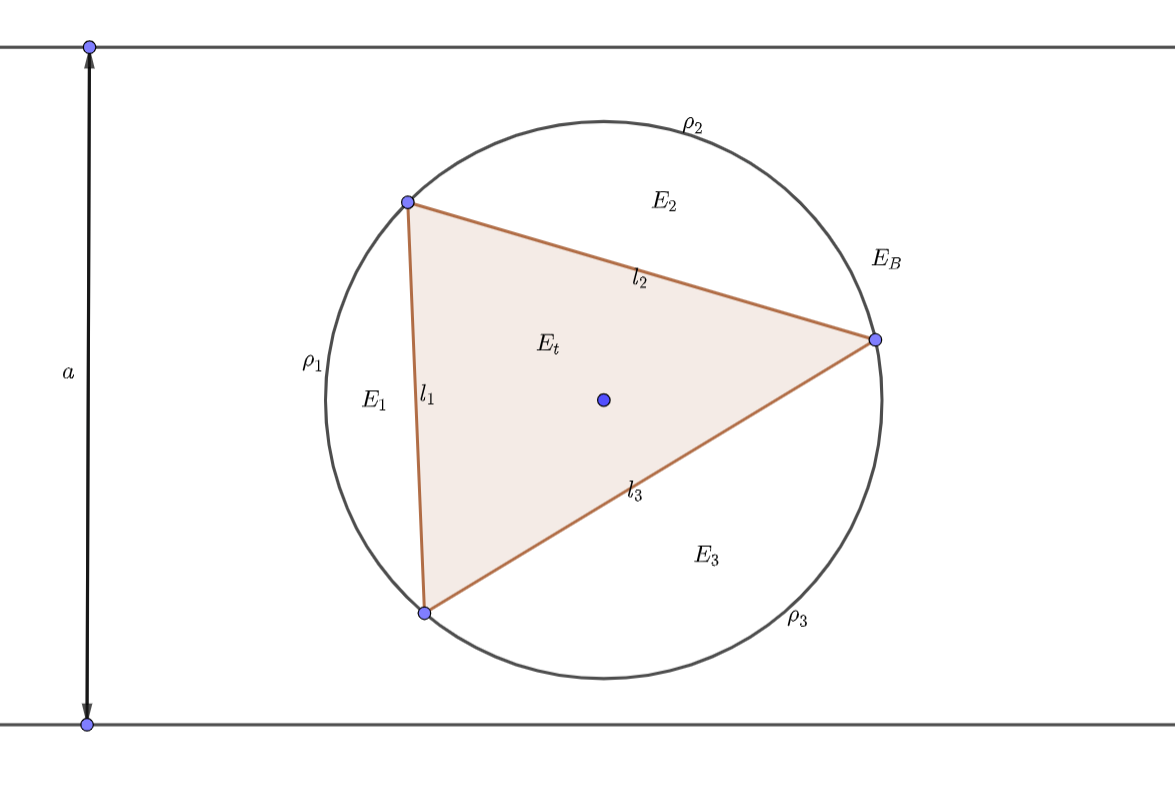
\includegraphics[width=0.8\textwidth]{figure.png}
}
\fi
\iffalse
% 表格模板
\renewcommand\arraystretch{0.8} % 设置表格高度为原来的0.8倍
\begin{table}[!htbp] % table标准
    \centering % 表格居中
    \begin{tabular}{p{1cm}<{\centering}p{1cm}<{\centering}p{3cm}<{\centering}p{5cm}<{\centering}} % 设置表格宽度
    %\begin{tabular}{cccc}
        \toprule
        $x_i$ & $f[x_1]$ & $f[x_i,x_{i+1}]$ & $f[x_i,x_{i+1},x_{i+2}]$ \\
        \midrule
        $x_0$ & $f(x_0)$ &                  &                          \\
        $x_0$ & $f(x_0)$ & $f'(x_0)$        &                          \\
        $x_0$ & $f(x_1)$ & $\frac{f(x_1)-f(x_0)}{x_1-x_0}$ & $\frac{f(x_1)-f(x_0)}{(x_1-x_0)^2}-\frac{f'(x_0)}{x_1-x_0}$\\
        \bottomrule
    \end{tabular}
\end{table}

\def\Log{\text{Log}} % 一个简单的宏定义
$\Log$ % 调用方法
\fi

\end{document}